\section{Differenzialrechnung}
Im Kapitel Differenzialrechnung werden wir die Themengebiete Extremwerte mit zwei Variablen, Extremwerte unter Nebenbedingungen betrachten und das Thema Homogenität wiederholen.
\subsection{Extremwertprobleme mit zwei Variablen}
Aus der eindimensionalen Differenzialrechnung wissen wir bereits,
dass
\begin{align*}
f^\prime(x) = 0
\end{align*}
als notwendige Bedingung für eine Extremstelle oder einen Sattelpunkt erfüllt sein muss.
Eine entsprechende Bedingung gibt es auch in der zweidimensionalen Differentialrechnung.\\
\index{stationäre Punkte!notwendiges Bed.}
\begin{mybox}{Notwendige Bedingung für stationäre Punkte}
Sei $f : \mathbb{R}^2 \to \mathbb{R}$ gegeben. 
Die \textit{notwendige Bedingung} für eine stationäre/kritische Stelle ist durch
\begin{align*}
f_x(x,y) &= 0\\
f_y(x,y) &= 0
\end{align*}
gegeben.
Alternativ können wir diese Bedingung auch als
\begin{align*}
\mathrm{grad} f (x,y) 
= 
\begin{pmatrix}
f_x(x,y)\\
f_y(x,y) 
\end{pmatrix}
= 
\textbf{0}
\end{align*}
schreiben.
\end{mybox}
Wir nennen dies einen stationären Punkt, da die Steigung Null beträgt.
Die Tangentialebene liegt also horizontal.
Hiermit können wir jedoch noch nicht mit Sicherheit sagen, ob es sich um ein Minimum,Maximum oder einen Sattelpunkt handelt.\\
\index{stationäre Punkte!hinreichende Bed.}
\begin{mybox}{Hinreichende Bedingungen}
Sei $f : \mathbb{R}^2 \to \mathbb{R}$ gegeben und $(x_0,y_0) $ ein kritischer Punkt.
Dann ist
\renewcommand{\labelenumi}{\theenumi.}
\begin{enumerate}
\item
\index{Minimum}
$f(x_0,y_0)$ ein \textit{Minimum}, falls
\begin{align*}
f_{xx}(x_0,y_0) > 0, \ f_{yy}(x_0,y_0) > 0, \ \text{und} \ f_{xx}(x_0,y_0)f_{yy}(x_0,y_0) - (f_{xy}(x_0,y_0))^2  > 0.
\end{align*}

\item
\index{Maximum}
$f(x_0,y_0)$ ein \textit{Maximum}, falls
\begin{align*}
f_{xx}(x_0,y_0) < 0, \ f_{yy}(x_0,y_0) < 0, \ \text{und} \ f_{xx}(x_0,y_0)f_{yy}(x_0,y_0) - (f_{xy}(x_0,y_0))^2  > 0.
\end{align*}

\item
\index{Sattelpunkt}
$f(x_0,y_0)$ ein \textit{Sattelpunkt}, falls
\begin{align*}
f_{xx}(x_0,y_0)f_{yy}(x_0,y_0) - (f_{xy}(x_0,y_0))^2  < 0.
\end{align*}

\end{enumerate}
\end{mybox}
\newpage




\pgfplotsset{width=7cm,compat=1.5.1}

\begin{tikzpicture}
\begin{axis}[view/h=10,view/v=20,axis lines = none]
\addplot3[
surf,
% shader=interp,
shader=flat,
samples=30,
domain=-3:3,y domain=-2:2]
{x^2 + y^2};
\end{axis}
\end{tikzpicture}
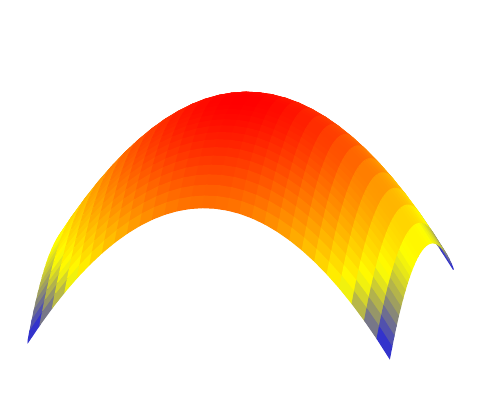
\begin{tikzpicture}
\begin{axis}[view/h=10,view/v=20,axis lines = none]
\addplot3[
surf,
% shader=interp,
shader=flat,
samples=30,
domain=-3:3,y domain=-2:2]
{-(x^2 + y^2)};
\end{axis}
\end{tikzpicture}
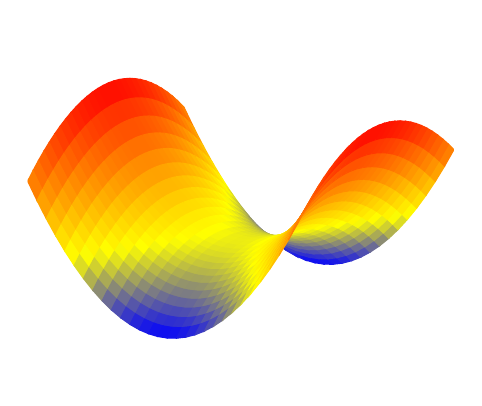
\begin{tikzpicture}
\begin{axis}[view/h=30,view/v=20,axis lines = none]
\addplot3[
surf,
% shader=interp,
shader=flat,
samples=30,
domain=-3:3,y domain=-2:2]
{x^2 -y^2};
\end{axis}
\end{tikzpicture}\\
Die Bilder veranschaulichen von links nach rechts:
Minimum, Maximum, Sattelpunkt.

\subsubsection*{Anwendungsbeispiel A}

Wir betrachten die Funktion $f(x,y) = x^2+ y^2 + 2y$.
Dann gilt
\begin{align*}
f_x(x,y) &= 2x\\
f_y(x,y) &= 2y+ 2
\end{align*}
für die partiellen Ableitungen.
Für stationäre Punkte muss die notwendige Bedingung 
\begin{align*}
f_x(x,y) &= 2x = 0 \ \Leftrightarrow \ x = 0\\
f_y(x,y) &= 2y +2 = 0 \ \Leftrightarrow \ 2y = -2 
\ \Leftrightarrow \ y = -1
\end{align*}
erfüllt sein.
Durch schnelles Nachrechnen sehen wir, dass $(0,-1)$ ein kritischer Punkt ist.
Für die Art des stationären Punktes benötigen wir noch die zweiten partiellen Ableitungen, welche durch
\begin{align*}
f_{xx}(x,y) &= 2\\
f_{yy}(x,y) &= 2\\
f_{xy}(x,y) &= 0
\end{align*}
gegeben sind.
Wir sehen, dass
\begin{align*}
f_{xx}(0,-1) > 0, \ f_{yy}(0,-1) > 0 , \ f_{xx}(0,-1) \cdot f_{yy}(0,-1) - (f_{xy}(0,-1))^2 > 0
\end{align*}
erfüllt ist.
Damit is unser stationärer Punkt $(0,-1)$ ein Minimum.
\newpage
\subsubsection*{Anwendungsbeispiel B}
Sei $f \ : \ \mathbb{R} \times (-5, \infty) \to \mathbb{R}$ eine Funktion zweier reeller Variablen definiert durch:
\begin{equation*}
f(x,y)\ = \ x^2 + 3 x y + 16 \ln(y+5).
\end{equation*}
Sei $g \ : \ R_f \to \mathbb{R}$ eine stetig differenzierbare Funktion einer reellen Variablen mit $g^\prime(x) > 0$
für alle $x \in R_f$, wobei $R_f$ der Wertebereich von $f$ ist.
Schließlich sei die Komposition $h$ gegeben als
\begin{equation*}
h \ : \ D_f \to \mathbb{R}, \quad (x,y) \mapsto h(x,y) = g(f(x,y)),
\end{equation*}
$D_f$ ist dabei das Definitionsgebiet von $f$.
\\
\\
Untersuchen Sie die Funktion $h$ auf stationäre Punkte, d.h., Maxima, Minima und Sattelpunkte.
\\
\\
\textbf{Hinweis:} \\
Dank der Eigenschaft von $g$ ist es möglich, das Problem in handhabbare Form zu bringen.\\

\textbf{Lösung:}
\begin{mdframed}
\underline{\textbf{Vorgehensweise:}}
\renewcommand{\labelenumi}{\theenumi.}
\begin{enumerate}
\item Verwende die gegebenen Eigenschaften, um das Problem zu strukturieren.
\item Finde die stationären Punkte von $h$.
\item Bestimme die Art des stationären Punkts.
\end{enumerate}
\end{mdframed}

\underline{1. Verwende die gegebenen Eigenschaften, um das Problem zu strukturieren}\\
Nach Voraussetzung ist $g^\prime(x) > 0$ für alle $x \in R_f$.
Die \textit{notwendige} Bedingung für stationäre Punkte ist, dass die partiellen Ableitungen von $h$ gleichzeitig Null sind.
Mathematisch können wir dies durch
\begin{align*}
h_x(x, y) = 0 \qquad 
h_y(x, y) = 0
\end{align*}
ausdrücken.
Die Punkte $(x, y)$, welche diese Bedingung erfüllen, nennen wir stationäre Punkte.
Wegen $g^\prime(x) > 0 $ gilt
\begin{align*}
h_x(x, y) &=  g^\prime(f(x,y)) \cdot f_x(x,y) = 0
\Leftrightarrow
f_x(x,y) = 0\\
h_y(x,y) &= g^\prime(f(x,y)) \cdot f_y(x,y) = 0 
\Leftrightarrow
f_y(x,y) = 0.
\end{align*}
Dies kann man sich mithilfe der Kettenregel überlegen.
Die Kettenregel findet Anwendung bei verketteten Funktionen sprich, wenn eine Funktion eine äußere und eine innere Funktion hat.
Dies ist bei 
\begin{align*}
h(x,y) = g(f(x,y)) 
\end{align*}
gegeben. Hierbei ist $g$ die äußere und $f$ die innere Funktion.
Die Kettenregel funktioniert hier wie im eindimensionalen Fall.
Wenn wir partiell nach $x$ ableiten, behandeln wir $y$ als eine Konstante.
Damit genügt es die stationären Punkte von $f$ zu bestimmen, da diese mit denen von $h$ übereinstimmen.
Wegen $g^\prime(x) > 0 $ können $h_x$ und $h_y$ nur Null ergeben, wenn $f_x$ bzw. $f_y$ Null ergeben.\\
\newpage
\underline{2. Finde die stationären Punkte von $h$}\\
Zunächst bestimmen wir durch
\begin{equation*}
\begin{split}
f_x(x,y) &= 2x + 3y \\
f_y(x,y) &= 3x + 16 (y+5)^{-1} = 3x + \frac{16}{y+5}
\end{split}
\end{equation*}
die ersten partiellen Ableitungen von $f$.
Diese müssen nun die \textit{notwendigen} Bedingungen
\begin{equation*}
f_x(x,y) = 0 \ \text{und} \ f_y(x,y) = 0
\end{equation*}
erfüllen. Dies führt zu dem Gleichungssystem
\begin{equation*}
\begin{split}
f_x(x,y) &= 2x + 3y = 0\\
f_y(x,y) &=  3x + \frac{16}{y+5} = 0.
\end{split}
\end{equation*}
Durch Umformen der ersten Gleichung erhalten wir mit
\begin{equation*}
2x + 3y = 0 
\Leftrightarrow
3y = -2x
\Leftrightarrow
y = -\frac{2}{3} x 
\end{equation*}
eine Darstellung für $y$.
Wir lösen die Gleichung durch Einsetzen in die Mitternachtsformel:
\begin{equation*}
\begin{split}
&3x + \frac{16}{y+5} = 3x + \frac{16}{-\frac{2}{3}x+5} = 0\\
\Leftrightarrow
&3x \left( -\frac{2}{3}x+5 \right) + 16 = -2 x^2 + 15 x + 16 = 0\\
\Leftrightarrow
&x_{\nicefrac{1}{2}}= \frac{- 15 \pm \sqrt{15^2 - 4 \cdot (-2) \cdot 16}}{2 \cdot(- 2)} 
= \frac{15 \pm \sqrt{353}}{4}\\
\Rightarrow
&x_1 = \frac{15 - \sqrt{353}}{4}, \quad
x_2 = \frac{15 + \sqrt{353}}{4}
\end{split}
\end{equation*}
Wir setzen nun $x_1$ und $x_2$ in die Gleichung $y = -\frac{2}{3} x$ ein und bestimmen so die möglichen stationären Punkte:
\begin{equation*}
\begin{split}
x_1  = \frac{15 - \sqrt{353}}{4}
&\Rightarrow
y_1 = -\frac{2}{3} x_1 = \frac{-15 + \sqrt{353}}{6}
\Rightarrow
P_1 = \left( \frac{15 - \sqrt{353}}{4}, \frac{-15 + \sqrt{353}}{6} \right)
\\
x_2  = \frac{15 + \sqrt{353}}{4}
&\Rightarrow
y_2 = -\frac{2}{3} x_2 = \frac{-15 - \sqrt{353}}{6}
\Rightarrow
P_2 = \left( \frac{15 + \sqrt{353}}{4}, \frac{-15 - \sqrt{353}}{6} \right).
\end{split}
\end{equation*}
Wir können den Punkt $P_2$ direkt ausschließen, da dieser sich nicht in dem Definitionsgebiet von $f$ befindet.
Dies können wir an
\begin{align*}
\frac{-15 - \sqrt{353}}{6} < -5
\end{align*}
erkennen.
Unser stationärer Punkt ist also durch
\begin{align*}
P_1 = \left( \frac{15 - \sqrt{353}}{4}, \frac{-15 + \sqrt{353}}{6} \right)
\end{align*}
gegeben.\\

\newpage

\underline{3. Bestimme die Art des stationären Punkts}\\
Auch hier reicht es wieder $f$ zu untersuchen.
Zunächst betrachten wir die \textit{hinreichenden} Bedingungen für Maxima, Minima und Sattelpunkte.\\

\begin{mybox}{Hinreichende Bedingungen}
Sei $f : \mathbb{R}^2 \to \mathbb{R}$ gegeben und $(x_0,y_0) $ ein kritischer Punkt.
Dann ist
\renewcommand{\labelenumi}{\theenumi.}
\begin{enumerate}
\item
\index{Minimum}
$f(x_0,y_0)$ ein \textit{Minimum}, falls
\begin{align*}
f_{xx}(x_0,y_0) > 0, \ f_{yy}(x_0,y_0) > 0, \ \text{und} \ f_{xx}(x_0,y_0)f_{yy}(x_0,y_0) - (f_{xy}(x_0,y_0))^2  > 0.
\end{align*}

\item
\index{Maximum}
$f(x_0,y_0)$ ein \textit{Maximum}, falls
\begin{align*}
f_{xx}(x_0,y_0) < 0, \ f_{yy}(x_0,y_0) < 0, \ \text{und} \ f_{xx}(x_0,y_0)f_{yy}(x_0,y_0) - (f_{xy}(x_0,y_0))^2  > 0.
\end{align*}

\item
\index{Sattelpunkt}
$f(x_0,y_0)$ ein \textit{Sattelpunkt}, falls
\begin{align*}
f_{xx}(x_0,y_0)f_{yy}(x_0,y_0) - (f_{xy}(x_0,y_0))^2  < 0.
\end{align*}
\end{enumerate}
\end{mybox}
Wir bestimmen nun die zweiten partiellen Ableitungen von $f$.
Es gilt
\begin{equation*}
\begin{split}
f_{xx}(x,y)  &= 
\frac{\partial}{\partial \mathrm{x}} (2x + 3y) = 2
 \\
f_{xy}(x,y)  &=
= \frac{\partial}{\partial \mathrm{y}} (2x + 3y) 
= 3 \\
f_{yy}(x,y) &= 
\frac{\partial}{\partial \mathrm{y}} \left(3x + \frac{16}{y+5} \right)
=
\frac{\partial}{\partial \mathrm{y}} \left(3x + 16 \cdot (y+5)^{-1} \right)
= 16 \cdot (-1)\cdot(y+5)^{-2}
- \frac{16}{(y+5)^2}.
\end{split}
\end{equation*}
Wir sehen, dass $f_{xx}(x,y) > 0$ für alle $(x,y) \in D_f$ gilt. 
Es gilt auch $f_{yy}(x,y) < 0 $ für alle $(x,y) \in D_f$.
Damit ist 
\begin{equation*}
\underbrace{f_{xx}(x,y)}_{>0} \underbrace{f_{yy} (x,y)}_{< 0 } - \underbrace{(f_{xy}(x,y))^2}_{>0} < 0
\end{equation*}
für alle $(x,y) \in D_f$ gegeben.
Somit ist $P_1 $ ein Sattelpunkt.

\newpage


\subsection{Gradient}

\begin{mybox}{Definition}\index{Gradient}
Sei $f : \mathbb{R}^2 \to \mathbb{R}$ gegeben.
Dann ist der \textit{Gradient} durch
\begin{align*}
\mathrm{grad} f(\textbf{x}) = 
\mathrm{grad} f(x,y) :=
\begin{pmatrix}
f_x(x,y)\\
f_y(x,y)
\end{pmatrix}
\end{align*}
definiert.
Damit ist der Gradient der Vektor der partiellen Ableitungen.
\end{mybox}

\begin{figure}[H]
\centering
\includegraphics[scale=0.5]{sections/pics/gradient.png}
\end{figure}
Den Graph einer Funktion der Form $f : \mathbb{R}^2 \to \mathbb{R} $ können wir uns als ein Gebirge vorstellen. 
Der Gradient im Punkt $\textbf{x}$ liefert uns die Richtung des stärksten Anstiegs.
Die blauen Pfeile in der Ebene sind die Gradienten an den entsprechenden Punkten.
Wir wissen also mit dem Gradienten, in welche Richtung wir den \glqq Berg\grqq~am schnellsten besteigen können.
\\
\begin{mybox}{Wichtige Eigenschaft}
\begin{center}
$\mathrm{grad} f(x,y) = \ \text{\glqq Richtung des größten Anstiegs von $f$ in $(x,y)$\grqq}$
\end{center}
\end{mybox}
\subsubsection*{Anwendungsbeispiel A}
Sei $f(x,y) = -x^2 + 3 y^2 -5$. Dann gilt:
\begin{align*}
\mathrm{grad} f(x,y) = 
\begin{pmatrix}
f_x(x,y)\\
f_y(x,y)
\end{pmatrix}
= 
\begin{pmatrix}
-2x\\
6 y
\end{pmatrix}
\end{align*}
\newpage
\subsubsection*{Anwendungsbeispiel B}
Sei $f(x,y) = \sin(x) \cdot \cos(y)$.\\
Bestimmen Sie die Richtung des größten Anstiegs im Punkt $(0,\pi)$.\\
\\
Es gilt:
\begin{align*}
\mathrm{grad} f(x,y) = 
\begin{pmatrix}
f_x(x,y)\\
f_y(x,y)
\end{pmatrix}
=
\begin{pmatrix}
\cos(x) \cdot \cos(y)\\
-\sin(x) \cdot \sin(y)
\end{pmatrix}
\end{align*} 
Damit folgt:
\begin{align*}
\mathrm{grad} f(0,\pi)
=
\begin{pmatrix}
\cos(0) \cdot \cos(\pi)\\
-\sin(0) \cdot \sin(\pi)
\end{pmatrix}
=\begin{pmatrix}
1 \cdot (-1)\\
0 \cdot 0
\end{pmatrix}
=
\begin{pmatrix}
-1\\
0
\end{pmatrix}
\end{align*}
Damit ist $\begin{pmatrix} -1 & 0\end{pmatrix}^\top$ die Richtung des größten Anstiegs im Punkt $(0, \pi)$ von $f$.\\

\subsubsection*{Anwendungsbeispiel C}
Gegeben sei die Funktion zweier reeller Variablen 
$f \ : \ \mathbb{R}\times \mathbb{R} \to \mathbb{R}$ definiert durch:
\begin{equation*}
f(x,y) = e^{2x^2+y^3 +3x +3y}.
\end{equation*}
Bestimmen Sie die Gleichung (allgemeine Form) einer Ebene $\beta$ so,
dass der Vektor $\textbf{u} = (x_0,y_0,z_0)^\top$ orthogonal zu $\beta$ ist,
wobei $(x_0,y_0)^\top = \textbf{grad} f(0,0)$ und $z_0 = f(0,0)$ gilt.
\\
\\
\textbf{Lösung:}
\begin{mdframed}
\underline{\textbf{Vorgehensweise:}}
\renewcommand{\labelenumi}{\theenumi.}
\begin{enumerate}
\item Stelle eine passende Ebenengleichung auf und berechne die fehlenden Parameter.
\end{enumerate}
\end{mdframed}

\underline{1. Stelle eine passende Ebenengleichung auf und berechne die fehlenden Parameter}\\
Da der Vektor $\textbf{u} = (x_0,y_0,z_0)^\top$ orthogonal auf $\beta$ ist, ist $\textbf{u}$ ein Normalenvektor.
Damit können wir $\beta$ durch
\begin{align*}
\beta \ : \ x_0 x + y_0 y + z_0 z + d  = 0, \qquad d \in \mathbb{R}
\end{align*}
beschreiben.
Wir müssen also nur noch $\text{u}$ bestimmen.
Es gilt  
\begin{align*}
\textbf{grad} f(x,y) = e^{2x^2+y^3 +3x +3y} 
\begin{pmatrix}
4 x+ 3\\
3 y^2 + 3 
\end{pmatrix}
\end{align*}
für den Gradienten von $f$.
Durch
\begin{align*}
\textbf{grad} f(0 ,0)&=
e^0
\begin{pmatrix}
3\\
3
\end{pmatrix}
=
\begin{pmatrix}
3\\
3
\end{pmatrix} \\
f(0,0) &= e^0 = 1
\end{align*}
erhalten wir $(x_0,y_0,z_0)^\top = ( 3, 3,1)^\top$.
Damit haben wir durch
\begin{align*}
\beta \ : \ 3 x + 3 y + 1 z + d, \qquad d \in \mathbb{R}
\end{align*}
die allgemeine Form von $\beta$ gegeben.



\newpage
\subsection{Extremwerte unter Nebenbedingungen}
Wir haben eine Funktion mit $f : \mathbb{R}^2 \to \mathbb{R}$ gegeben.
Nun interessieren uns die Extrempunkte unter der Bedingung, dass 
\begin{align*}
\varphi(x,y) = 0
\end{align*}
erfüllt ist.
Dieses $\varphi$ nennen wir \textit{Nebenbedingung}.
Wichtig ist, dass die Nebenbedingung in der Aufgabenstellung beispielsweise durch
\begin{align*}
x = -y
\end{align*}
geben sein kann.
Durch die Umformung
\begin{align*}
x = -y 
\Leftrightarrow
\varphi(x,y) = x + y = 0
\end{align*}
erhalten wir dann die erforderliche Form.\\
\index{Substitutionsmethode}
\begin{mybox}{Substitutionsmethode}
Gegeben sei eine Funktion $f : \mathbb{R}^2 \to \mathbb{R}$ und
die Nebenbedingung $\varphi(x,y) = 0$.
Wenn es möglich ist, die Nebenbedingung durch
\begin{align*}
\varphi(x,y) = 0 \Leftrightarrow
y = g(x) 
\end{align*}
oder 
\begin{align*}
\varphi(x,y) = 0 \Leftrightarrow
x = g(y) 
\end{align*}
nach einer Variablen umzustellen, können wir das Extremwertproblem durch
Zurückführen auf die eindimensionale Differenzialrechnung lösen.
Durch Einsetzen von $y=g(x)$ erhalten wir mit
\begin{align*}
\tilde{f}(x) := f(x,y) = f(x,g(x))
\end{align*}
oder
\begin{align*}
\tilde{f}(y) := f(x,y) = f(g(y),y)
\end{align*}
das eindimensionale Extremwertproblem.
\end{mybox}
Dieses Verfahren nennen wir \textit{Substitutionsmethode}.
Da bei diesem Verfahren eine Variable verloren geht, wird ebenfalls der Name 
\textit{Variablenreduktion} oder \textit{Reduktionsmethode} verwendet.
Wann können wir dieses Verfahren anwenden?
Im Prinzip immer, wenn wir eindeutig nach einer Variablen auflösen können.\\ \\
Wir betrachten die Nebenbedingung
\begin{align*}
\varphi(x,y) = 2x -4y = 0.
\end{align*}
Diese lässt sich durch
\begin{align*}
2x - 4 y = 0 
\Leftrightarrow
x = 2y
\Leftrightarrow
y = \frac{1}{2} x
\end{align*}
eindeutig nach beiden Variablen umformen.
\newpage
Dies ist bei der Nebenbedingung
\begin{align*}
\varphi(x,y) = x^2 + y = 0
\end{align*}
nicht für beide Variablen möglich.
Durch 
\begin{align*}
y = -x^2 
\end{align*}
erhält man eine eindeutige Zuordnung für die $y $-Variable.
Jedoch ist wegen
\begin{align*}
x^2 + y = 0
\Leftrightarrow
x = \pm \sqrt{-y}
\end{align*}
keine eindeutige Zuordnung für die $x$-Variable möglich.\\

Da das Umformen nach einer Variablen nicht immer möglich ist, betrachten wir nun das \textit{Lagrange-Verfahren}.
\index{Lagrangeverfahren}
\begin{mybox}{Lagrangefunktion}
\index{Lagrangefunktion}
Geben sei eine Funktion $f : \mathbb{R}^2 \to \mathbb{R}$ und eine Nebenbedingung 
$\varphi(x,y) = 0$.
Dann bezeichnen wir 
\begin{align*}
F(x,y,\lambda) = f(x,y) + \lambda \varphi(x,y) 
\end{align*}
als \textit{Lagrangefunktion}.
\end{mybox}
\ \\
Doch wie finden wir nun mit dieser Funktion Extremwerte unter der Nebenbedingung?
Da dies eine mehrdimensionale Funktion ist, müssen auch alle partiellen Ableitungen gleichzeitig Null sein.\\

\begin{mybox}{Notwendige Bedingung für die Lagrangefunktion}
\index{Lagrangefunktion!notwendige Bed.}
Die notwendige Bedingung für Extremstellen unter der Nebenbedingung $\varphi(x,y) = 0$
ist durch
\begin{align*}
F_x(x,y,\lambda )&= 0\\
F_y(x,y,\lambda) &= 0\\
F_\lambda(x,y,\lambda) &= 0
\end{align*}
gegeben.
Die Punkte, welche diese Bedingung erfüllen, nennen wir wieder \textit{kritische/stationäre} Punkte.
\end{mybox}
\ \\
Wir können das Vorgehen hier in drei Schritte unterteilen:
\begin{mybox}{Vorgehensweise:}

Schritt 1: Aufstellen der Lagrangefunktion\\
Schritt 2: Bilden der ersten partiellen Ableitung nach $x$, $y$ und $\lambda$.\\
Schritt 3: Lösen des Gleichungssystem der notwendigen Bedingung für die Lagrangefunktion.

\end{mybox}
\newpage
\subsubsection*{Anwendungsbeispiel A}
Bestimmen Sie die Extrempunkte der Funktion
\begin{align*}
f(x,y) = x^2 +y^2
\end{align*}
unter der Nebenbedingung $\varphi(x,y) = x +4 y -2$.\\
\\
\underline{1. Aufstellen der Lagrangefunktion}\\
Die Lagrangefunktion ist durch
\begin{align*}
F(x,y,\lambda) = f(x,y) + \lambda \varphi(x,y) 
= x^2 +y^2 + \lambda(x +4 y -2).
\end{align*}
gegeben.\\
\\
\underline{2. Bilden der ersten partiellen Ableitung nach $x$, $y$ und $\lambda$}\\
Es gilt
\begin{align*}
F_x(x,y,\lambda) &= 2x + \lambda\\
F_y(x,y,\lambda) &= 2y + 4 \lambda\\
F_\lambda(x,y,\lambda) &= x+ 4y -2
\end{align*}
für die partiellen Ableitungen.\\
\\
\underline{3. Lösen des Gleichungssystem der notwendigen Bedingung für die Lagrangefunktion}\\
Nun gilt
\begin{align*}
F_x(x,y,\lambda) &= 2x + \lambda\ = 0 
\Leftrightarrow
\lambda = -2x\\
F_y(x,y,\lambda) &= 2y + 4 \lambda = 0
\Leftrightarrow 
\lambda = - \frac{1}{2}y\\
\Rightarrow
-2x &= - \frac{1}{2} y
\Leftrightarrow
y = 4 x,
\end{align*}
wodurch wir $\lambda$ eliminiert haben.
Setzen wir $y = 4x $ in die letzte Gleichung ein, erhalten wir durch
\begin{align*}
F_\lambda(x,y,\lambda) &= x +4y -2 = x + 16 x -2 = 0\\
\Leftrightarrow
x &= \frac{2}{17}
\Leftrightarrow
y = 4x = 4 \cdot \frac{2}{17} = \frac{8}{17} 
\end{align*}
den kritischen Punkt $\left( \frac{2}{17}, \frac{8}{17} \right)$.\\
\\
\begin{mybox}{Hinreichende Bedingung für Lagrangefuntion}
\index{Lagrangefunktion!hinreichende Bed.}
\renewcommand{\labelenumi}{\theenumi.}
\begin{enumerate}
\item
Falls
\begin{align*}
2 \varphi_x(x,y)\varphi_y(x,y) F_{xy}(x,y,\lambda)
-F_{xx}(x,y,\lambda) \varphi_y^2(x,y) 
- F_{yy}(x,y,\lambda)\varphi_x^2(x,y) < 0
\end{align*}
gilt, liegt ein \textit{Minimum} vor.
\item
Falls
\begin{align*}
2 \varphi_x(x,y)\varphi_y(x,y) F_{xy}(x,y,\lambda)
-F_{xx}(x,y,\lambda) \varphi_y^2(x,y) 
- F_{yy}(x,y,\lambda)\varphi_x^2(x,y) > 0
\end{align*}
gilt, liegt ein \textit{Maximum} vor.
\end{enumerate}
\end{mybox}

\subsubsection*{Fortsetzung des Anwendungsbeispiels A}
Zunächst bestimmen wir mit
\begin{align*}
\varphi_x(x,y) &= 1 \\
\varphi_y(x,y) &= 4\\
F_{xx}(x,y,\lambda) &= 2 \\
F_{yy}(x,y,\lambda) &= 2\\
F_{xy}(x,y,\lambda) &= 0
\end{align*}
die für die hinreichende Bedingung notwendigen Ableitungen.
Mit $(x,y) :=  \left( \frac{2}{17}, \frac{8}{17} \right)$ folgt dann durch
\begin{align*}
&2 \varphi_x(x,y)\varphi_y(x,y) F_{xy}(x,y,\lambda)
-F_{xx}(x,y,\lambda) \varphi_y^2(x,y) 
- F_{yy}(x,y,\lambda)\varphi_x^2(x,y)\\
=
&2 \cdot 1 \cdot 4 \cdot 0 - 2 \cdot 4^2 - 2 \cdot 1^2 
=
- 32 - 2 = -34 < 0,
\end{align*}
dass es sich bei dem Punkt $\left( \frac{2}{17}, \frac{8}{17} \right)$ um ein Minimum von $f$ unter der Nebenbedingung $\varphi$ handelt.\\
\\

\subsubsection*{Anwendungsbeispiel B}
Ein Konsument \textit{maximiert} seine Nutzenfunktion $u(c_1,c_2)$ in den Einheiten $c_1$ und $c_2$
der Güter 1 und 2 definiert durch:
\begin{equation*}
u \ : \ \mathbb{R}_+ \times \mathbb{R}_+ \to \mathbb{R},
\quad (c_1,c_2) \mapsto u(c_1,c_2) = c_1^{0.6} c_2^{0.4}
\end{equation*}
über die Wahl des Konsumbündels $(c_1^\star,c_2^\star)$.
Die Preise der Güter 1 und 2 sind $p_1 \ = \ 3$ beziehungsweise $p_2 \ = \ 4$,
und das Budget, welches \textit{vollständig} genutzt wird, beträgt $e = 15$.
\\
Bestimmen Sie die stationären Punkte des Maximierungsproblems des Konsumenten, 
d.h., Kandidaten für das optimale Konsumbündel $(c_1^\star,c_2^\star)$.
\\
\\
\textbf{Hinweis:}\\ 
Eine Abklärung, ob es sich bei den stationären Punkten tatsächlich um Maxima handelt, wird nicht verlangt.
\\
\\
\textbf{Lösung:}
\begin{mdframed}
\underline{\textbf{Vorgehensweise:}}
\renewcommand{\labelenumi}{\theenumi.}
\begin{enumerate}
\item Formuliere das Optimierungsproblem mathematisch.
\item Löse die Aufgabe mithilfe der Lagrange Methode.
\item Alternative Rechenmethode.
\end{enumerate}
\end{mdframed}
\underline{1. Formuliere das Optimierungsproblem mathematisch}\\
Unser Ziel ist es, die Funktion
\begin{equation*}
u(c_1,c_2) = c_1^{0.6}c_2^{0.4}
\end{equation*}
unter der Nebenbedingung
\begin{equation*}
p_1 c_1 + p_2 c_2 = e \Rightarrow
\varphi(c_1,c_2) = p_1 c_1 + p_2 c_2 - e = 3 c_1 + 4 c_2 - 15 = 0
\end{equation*}
zu maximieren.
\\
\\
\underline{2. Löse die Aufgabe mithilfe der Lagrange Methode}\\
Zunächst bietet es sich bei Extremwertaufgaben unter Nebenbedingungen an, die Lagrange Methode zu verwenden
Die Nebenbedingung
\begin{equation*}
\varphi(c_1,c_2) = 3 c_1 + 4 c_2 - 15 = 0
\end{equation*}
besitzt nur lineare Terme.
Das heißt, wir können diese explizit nach $c_1$ bzw. $c_2$ auflösen.
Durch diese Umformung erhalten wir aus $u$ eine Funktion, welche von einer Variablen abhängt.
Beide Methoden sind in etwa gleich schwer, jedoch funktioniert die zweite Methode nicht immer.
\\
\\ 
Wir definieren durch
\begin{equation*}
F(c_1,c_2,\lambda) = u(c_1,c_2) + \lambda \varphi(c_1,c_2)
= c_1^{0.6}c_2^{0.4} + \lambda \cdot( 3 c_1 + 4 c_2- 15)
\end{equation*}
die Lagrange-Funktion.
Die notwendige Bedingung für Extremstellen unter unserer Nebenbedingung ist,
dass die partiellen Ableitungen der Lagrange-Funktion gleichzeitig Null sind.
Durch
\begin{align*}
F_{c_1}(c_1,c_2,\lambda) &= 0.6 c_1^{-0.4} c_2^{0.4} + 3 \lambda\\
F_{c_2}(c_1,c_2, \lambda) &= 0.4 c_1^{0.6} c_2^{-0.6} + 4 \lambda \\
F_{\lambda}(c_1,c_2,\lambda) &=\varphi(c_1,c_2) = 3 c_1 + 4 c_2 -15 
\end{align*}
erhalten wir die partiellen Ableitungen.
Wir müssen nun das Gleichungssystem
\newcounter{eq}
\setcounter{eq}{0}
\begin{align}
0.6 c_1^{-0.4} c_2^{0.4} + 3 \lambda = 0  \tag{\text{\Roman{eq}}}\stepcounter{eq}\\
0.4 c_1^{0.6} c_2^{-0.6} + 4 \lambda = 0  \tag{\text{\Roman{eq}}}\stepcounter{eq}\\
3 c_1 + 4 c_2 -15 = 0 \tag{\text{\Roman{eq}}}\stepcounter{eq}
\end{align}
lösen. 
Die Gleichungen (I) und (II) liefern uns durch
\begin{align}
0.6 c_1^{-0.4} c_2^{0.4} + 3 \lambda &= 0 
\Leftrightarrow 
3 \lambda = -0.6 c_1^{-0.4} c_2^{0.4} 
\Leftrightarrow
3 \lambda= -0.6 \frac{c_2^ {0.4}}{c_1^{0.4}}
\Leftrightarrow
3 \lambda= -0.6 \left( \frac{c_2}{c_1} \right)^{0.4}
\tag{\text{\Roman{eq}}}\stepcounter{eq}\\
0.4 c_1^{0.6} c_2^{-0.6} + 4 \lambda &= 0 
\Leftrightarrow 
4 \lambda = - 0.4 c_1^{0.6} c_2^{-0.6} 
\Leftrightarrow
4 \lambda = -0.4  \frac{c_1^{0.6}}{c_2^{0.6}}
\Leftrightarrow
4 \lambda=- 0.4 \left( \frac{c_1}{c_2} \right)^{0.6}
\tag{\text{\Roman{eq}}}\stepcounter{eq}    
\end{align}
zwei neue Gleichungen.
Wegen $c_1, c_2 > 0 $ sehen wir, dass $\lambda \neq 0 $ gilt.
Also können wir (IV) durch (V) teilen.
Damit gilt
\begin{equation*}
\begin{split}
\frac{3 \lambda }{4 \lambda} 
&= \frac{-0.6 \left( \frac{c_2}{c_1} \right)^{0.4}}{- 0.4 \left( \frac{c_1}{c_2} \right)^{0.6}}
= \frac{3}{2} \cdot \frac{c_2^{0.4} c_2^{0.6}}{c_1^{0.6} c_1^{0.4}}
= \frac{3}{2} \frac{c_2}{c_1}\\
\Rightarrow
\frac{3 \lambda }{4 \lambda} &= \frac{3}{2} \frac{c_2}{c_1}
\Leftrightarrow
\frac{3  }{4 } = \frac{3}{2} \frac{c_2}{c_1}
\Leftrightarrow
6 c_1 = 12 c_2
\Leftrightarrow
c_1 = 2 c_2,
\end{split}
\end{equation*}
womit durch Gleichung (III)
\begin{equation*}
\begin{split}
3 c_1 + 4 c_2 - 15 &= 3 (2c_2) + 4 c_2 -15 = 10 c_2  -15 = 0 \\
\Leftrightarrow
10 c_2 &= 15 
\Leftrightarrow
c_2 = \frac{15}{10} = \frac{3}{2} = 1.5  
\end{split}
\end{equation*}
folgt.
Durch $c_1 = 2 c_2 $ wissen wir auch $c_1 = 3$.
Damit ist 
\begin{align*}
(c_1^\star, c_2^\star) = ( 3, 1.5)
\end{align*}
der einzige Kandidat für eine Extremstelle unter der Nebenbedingung $\varphi$.\\
\\
\underline{3. Alternative Rechenmethode}\\
Für die alternative Methode formen wir die Nebenbedingung $\varphi$ nach einer Variablen um
und substituieren diese in $u$.
Durch die Umformung 
\begin{equation*}
\begin{split}
\varphi(c_1,c_2) &= p_1 c_1 + p_2 c_2 -e = 3 c_1 + 4 c_2 - 15 = 0\\
\Leftrightarrow
3 c_1 &= 15 - 4 c_2 \\
\Leftrightarrow
c_1 &= 5 - \frac{4}{3} c_2
\end{split}
\end{equation*}
können wir $c_1 $ durch $c_2$ darstellen.
Damit erhalten wir mit 
\begin{equation}
U(c_2) = u( c_1 , c_2) 
= u\left( 5 - \frac{4}{3}c_2,c_2 \right) 
=\left( 5 - \frac{4}{3}c_2 \right)^{0.6} c_2^{0.4}
\end{equation}
eine Funktion, welche nur von der Variablen $c_2$ abhängt.
Wir müssen nun die Extrempunkte von $U$ finden. 
Hierfür lösen wir $U^\prime(c_2) = 0 $.
Zunächst gilt
\begin{equation*}
\begin{split}
U^\prime(c_2)
&= 0.6 \left( 5 - \frac{4}{3} c_2 \right)^{-0.4} \left( -\frac{4}{3} \right) c_2^{0.4}
+ 0.4 \left( 5 - \frac{4}{3} c_2 \right)^{0.6} c_2^{-0.6}\\
&= -\frac{4}{5} \left( 5 - \frac{4}{3} c_2 \right)^{-0.4}  c_2^{0.4}
+ \frac{2}{5} \left( 5 - \frac{4}{3} c_2 \right)^{0.6} c_2^{-0.6}\\
&= -\frac{4}{5} \left( \frac{1}{5 - \frac{4}{3} c_2 }\right)^{0.4}  c_2^{0.4}
+ \frac{2}{5} \left( 5 - \frac{4}{3} c_2 \right)^{0.6} \frac{1}{c_2}^{0.6}\\
&= - \frac{4}{5} \left( \frac{c_2}{5 - \frac{4}{3} c_2} \right)^{0.4}
+ \frac{2}{5} \left( \frac{5 - \frac{4}{3} c_2}{c_2}  \right)^{0.6}\\
&= - \frac{4}{5} \left( \frac{c_2}{5 - \frac{4}{3} c_2} \right)^{0.4}
+ \frac{2}{5} \left( \frac{c_2}{5 - \frac{4}{3} c_2} \right)^{0.4} \frac{5 - \frac{4}{3} c_2}{c_2}\\
&=
\left( \frac{c_2}{5 - \frac{4}{3} c_2} \right)^{0.4} \left( -\frac{4}{5} + \frac{2}{5} \frac{5 - \frac{4}{3} c_2}{c_2} \right)
\end{split}
\end{equation*}
mithilfe der Produkt und Kettenregel.
Die weiteren Umformungen helfen uns $U^\prime(c_2) = 0$ zu lösen.
Wegen $c_2 \neq 0 $ erhalten wir durch
\begin{equation*}
\begin{split}
U^\prime(c_2) = 0 
&\Leftrightarrow
\left( \frac{c_2}{5 - \frac{4}{3} c_2} \right)^{0.4} \left( -\frac{4}{5} + \frac{2}{5} \frac{5 - \frac{4}{3} c_2}{c_2} \right) = 0\\
&\Leftrightarrow
\left( -\frac{4}{5} + \frac{2}{5} \frac{5 - \frac{4}{3} c_2}{c_2} \right) = 0\\
&\Leftrightarrow
-\frac{4}{5} c_2 + \frac{2}{5}\left(5 -\frac{4}{3} c_2 \right) 
= 0 \\
& \Leftrightarrow 
-\frac{4}{5} c_2 + 2 - \frac{8}{15} c_2 = 0\\
&\Leftrightarrow
\left(- \frac{4}{5} - \frac{8}{15} \right) c_2 = -2\\
&\Leftrightarrow
-\frac{20}{15} c_2 = - 2 
\Leftrightarrow
c_2 = 1.5
\end{split}
\end{equation*}
das passende $c_2$.
Mit $c_1 = 5 - \frac{4}{3} c_2$ folgt auch $c_1 = 5 - \frac{4}{3 } \cdot \frac{3}{2} = 5 - 2 = 3$.
Damit ist auch bei dieser Methode
\begin{align*}
(c_1^\star , c_2^\star) = (3, 1.5)
\end{align*}
der einzige Kandidat für eine Extremstelle unter der Nebenbedingung $\varphi$.
\\
\\
Der Kandidat für das optimale Konsumbündel ist $(c_1^\star , c_2^\star) = (3, 1.5)$.

\newpage
\subsection{Homogene Funktionen}
\index{homogene Funktionen}
\begin{mybox}{Definition}
Eine Funktion $f : \mathbb{R}^2 \to \mathbb{R}$ heißt \textit{homogen} von Grad $k$,
falls
\begin{align*}
f(\lambda \cdot x, \lambda \cdot y) = \lambda^k f(x,y)
\end{align*}
für alle $\lambda \in \mathbb{R}$ erfüllt ist.
\end{mybox}

\subsubsection*{Anwendungsbeispiel A}
Gegeben sei die Funktion $f$ definiert durch
\begin{align*}
f(x,y) = \sqrt[5]{x^{3.4}y^{0.6}}+ \sqrt{x^{0.8}y^{0.8}} 
+ \sqrt[3]{x^{1.6}y^{1.6}}
\end{align*}
wobei $x >0$ und $y> 0$.
\renewcommand{\labelenumi}{(\alph{enumi})}
\begin{enumerate}
\item $f$ ist homogen vom Grad $0.6$.
\item $f$ ist homogen vom Grad $0.7$.
\item $f$ ist homogen vom Grad $0.8$.
\item $f$ ist nicht homogen.
	
\end{enumerate}
\ \\
\textbf{Lösung:}
\begin{mdframed}
\underline{\textbf{Vorgehensweise:}}
\renewcommand{\labelenumi}{\theenumi.}
\begin{enumerate}
\item Beweise, ob die Funktion homogen oder nicht homogen ist.
\end{enumerate}
\end{mdframed}

\underline{1. Beweise, ob die Funktion homogen oder nicht homogen ist}\\
%Wir wählen ein beliebiges $\lambda >0 $. 
%Für $\lambda = 0 $ erhalten wir die Gleichung $0 = 0$, wodurch wir diesen Fall direkt auschließen können.
Durch Einsetzen erhalten wir:
\begin{align*}
f( \lambda x, \lambda y ) 
&= \sqrt[5]{(\lambda x)^{3.4} (\lambda y)^{0.6}}
  + \sqrt{(\lambda x)^{0.8} (\lambda y)^{0.8}}
  + \sqrt[3]{(\lambda x)^{1.6} (\lambda y)^{1.6}}\\
&=  \sqrt[5]{\lambda^{3.4} x^{3.4} \lambda^{0.6} y^{0.6}}
  + \sqrt{\lambda^{0.8} x^{0.8} \lambda^{0.8} y^{0.8}}
  + \sqrt[3]{\lambda^{1.6} x^{1.6} \lambda^{1.6} y^{1.6}}\\
&=  \sqrt[5]{\lambda^{4} x^{3.4} y^{0.6}}
  + \sqrt{\lambda^{1.6} x^{0.8}  y^{0.8}}
  + \sqrt[3]{\lambda^{3.2} x^{1.6} y^{1.6}}\\
&=  \lambda^{0.8} \sqrt[5]{ x^{3.4} y^{0.6}}
  + \lambda^{0.8} \sqrt{ x^{0.8}  y^{0.8}}
  + \lambda^{\frac{3.2}{3}} \sqrt[3]{ x^{1.6} y^{1.6}}\\
&=  \lambda^{0.8} \left( \sqrt[5]{ x^{3.4} y^{0.6}}
  + \sqrt{ x^{0.8}  y^{0.8}}
  + \lambda^{\frac{3.2}{3} -0.8} \sqrt[3]{ x^{1.6} y^{1.6}} \right)
\end{align*}
$f$ ist damit nicht homogen.\\
\\
Somit ist Antwort (d) richtig.

\newpage
\subsubsection*{Anwendungsbeispiel B}
Gegeben sei die Funktion $f$ definiert durch
\begin{align*}
f(x,y) = x^{3.1} \sqrt{y} + 6 y^{3.5} \sqrt{ 5 x^{0.2}}
		+ x^a y^{2a}
\end{align*}
wobei $x > 0 $, $ y >0 $ und $a \in \mathbb{R}$.\\ \\
Für welchen Wert von $a$ ist $f$ homogen?
\renewcommand{\labelenumi}{(\alph{enumi})}
\begin{enumerate}
\item $a = 1$.
\item $a = 1.2$.
\item $a = 1.4$.
\item $f$ ist für kein $a \in \mathbb{R}$ homogen.
	
\end{enumerate}
\ \\
\textbf{Lösung:}
\begin{mdframed}
\underline{\textbf{Vorgehensweise:}}
\renewcommand{\labelenumi}{\theenumi.}
\begin{enumerate}
\item Rechne die Definition der Homogenität nach.
\end{enumerate}
\end{mdframed}

\underline{1. Rechne die Definition der Homogenität nach}\\
Durch Einsetzen erhalten wir:
\begin{align*}
f(\lambda x , \lambda y) 
&= (\lambda x )^{3.1} \sqrt{\lambda y}
	+ 6 (\lambda y)^{3.5} \sqrt{5 (\lambda x)^{0.2}}
	+(\lambda x)^a (\lambda y)^{2a}\\
&= \lambda^{3.1} x^{3.1}  \lambda^{0.5} \sqrt{ y}
	+ 6 \lambda^{3.5} y^{3.5} \sqrt{5 \lambda^{0.2} x^{0.2}}
	+\lambda^a x^a \lambda^{2a} y^{2a}\\
&= \lambda^{3.6} x^{3.1}  \sqrt{ y}
	+ 6 \lambda^{3.5} y^{3.5} \lambda^{0.1} \sqrt{5  x^{0.2}}
	+\lambda^{3a} x^a  y^{2a}\\
&= \lambda^{3.6} x^{3.1}  \sqrt{ y}
	+ 6 \lambda^{3.6} y^{3.5}  \sqrt{5  x^{0.2}}
	+\lambda^{3a} x^a  y^{2a}\\
&= \lambda^{3.6} \left( x^{3.1}  \sqrt{ y}
	+ 6 y^{3.5}  \sqrt{5  x^{0.2}}
	+\lambda^{3a - 3.6} x^a  y^{2a} \right)\\		
\end{align*}
Diese Funktion ist homogen, wenn $3a - 3.6 = 0$ gilt.
Mit 
\begin{align*}
&\ \ \ \ \ 3 a - 3.6 = 0\\
&\Leftrightarrow
3a = 3.6\\
&\Leftrightarrow
a = 1.2
\end{align*}
erhalten wir noch das dazu passende $a$.\\
\\
Somit ist Antwort (b) richtig.


